\section{RADS Framework}
\label{sec:framework} 

\begin{figure*}
  % {\epsfig{file = figures/RAIDS_framework, width = \textwidth, height=4cm}}
  \centering
     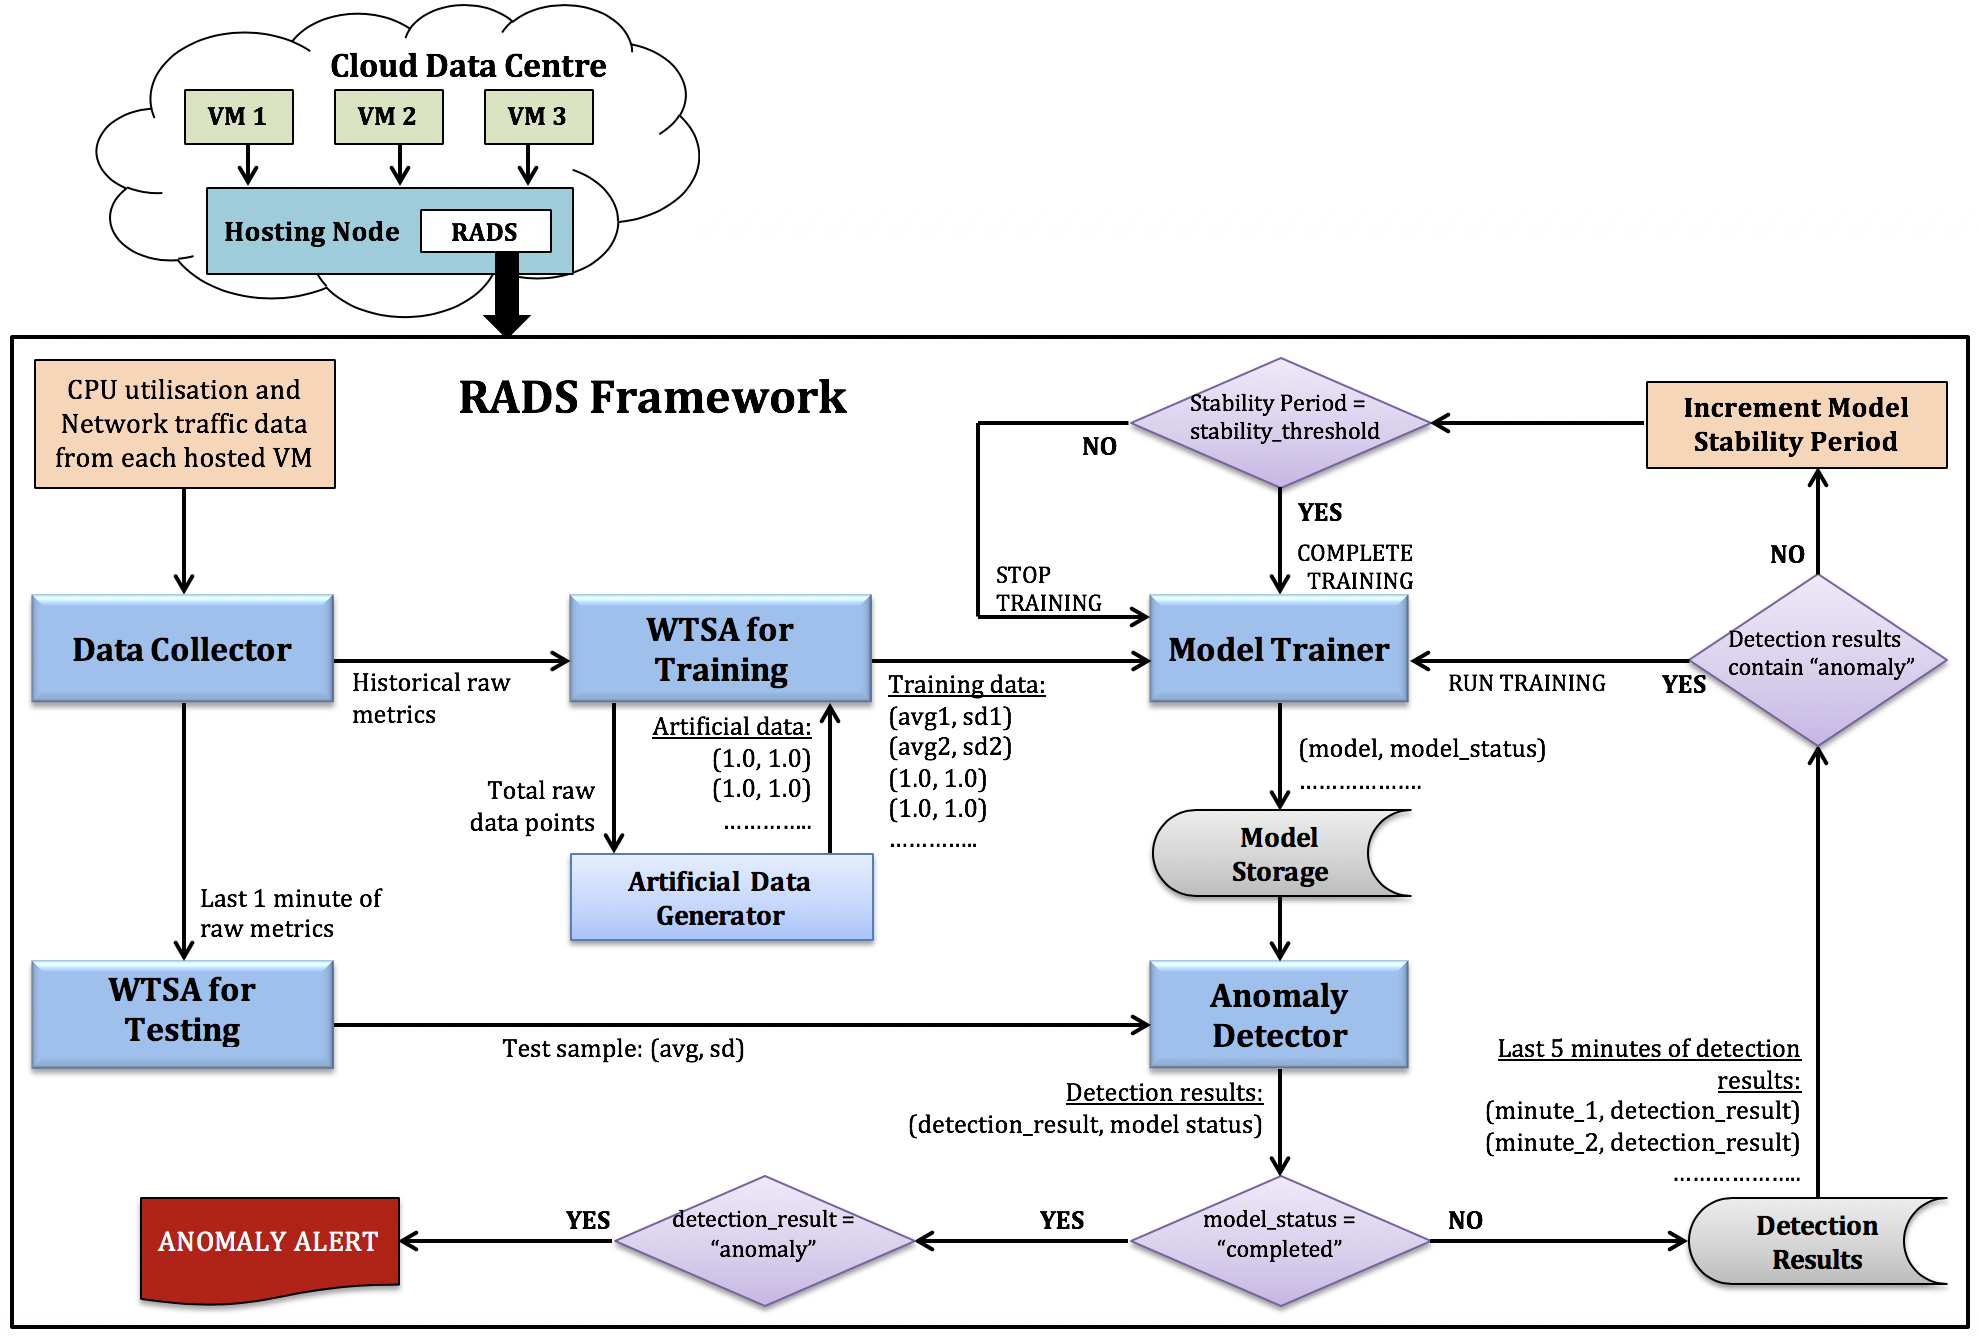
\includegraphics[width=0.9\textwidth]{figures/RADS_Framework}
   \caption{RADS framework}
  \label{fig:framework}
\end{figure*}
%\vfill

\noindent In this section we present the detailed framework of RADS. 
Figure~\ref{fig:framework} depicts the framework, which is designed to be implemented on each hosting node in a Cloud data centre locally, where it can monitor all the hosted VMs in order to detect the VM-level anomalies. % in their resource usage.
%Importantly, all the operations of RADS are in real-time in order to detect the anomalies as they appear.

\subsection{Data Collection}
\noindent RADS uses the \textit{Data Collector} module to collect the CPU utilisation and the network traffic (total size of network packets transmitted and received) metrics of each of the hosted VMs. The frequency of collecting these metrics is 5 seconds which allows capture of the CPU and network usage behaviour in a fine-grained manner.
The module runs virt-top\footnote{http://people.redhat.com/rjones/virt-top/} (a top-like utility for retrieving statistics of virtualised domains) on the hosting node for collecting the VM-level metrics. 
%\subsection{Window-based Time Series Analysis for Training}
%RADS processes the raw metrics before they are used as the training data for training the OCC models or as the test sample for detecting anomaly. RADSs uses two modules for this purpose: \textbf{Data Pre-processor for Training} which processes the historical raw metrics to prepare them as the training data and \textbf{Data Pre-processor for Testing} which processes the last one minute of raw metrics to prepare them as test sample. The modules consider window-based processing of the raw metrics.


%PRE-PROCESSING FOR TRAINING
%\vfill
\begin{algorithm}
\caption{Window-based Time Series Analysis (WTSA) For Training}
\label{raids_algorithm_pre-processing_1}
%\algnewcommand\algorithmicheadingA{\underline{\textbf{{Data Pre-processing}}}}
\algnewcommand\algorithmicinput{\textbf{input:}}
\algnewcommand\algorithmicoutput{\textbf{output:}}
\algnewcommand\algorithmicabb{\textbf{abbreviation:}}
%\algnewcommand\HEADINGA{\item[\algorithmicheadingA]}
\algnewcommand\INPUT{\item[\algorithmicinput]}
\algnewcommand\OUTPUT{\item[\algorithmicoutput]}
\algnewcommand\ABB{\item[\algorithmicabb]}

\begin{algorithmic}[1]
%\algnewcommand\algorithmicheadingAA{\underline{\textbf{{(a) Training Data Pre-processing}}}}
%\algnewcommand\HEADINGAA{\item[\algorithmicheadingAA]}
%\HEADINGAA
\INPUT $Raw_{historical}$ - historical raw metrics of N VMs; $DW$ - distribution window = 1 minute
\OUTPUT $INN_{training}$ - set of normalised input instances for training; total N sets for N VMs
%\OUTPUT $V_{training}$ - set of vectors as training data; total N sets for N VMs.
\ABB 
$avg = Average$; $sd = Standard Deviation$
\Statex
\For {\textbf{each} VM $vm_i$ \textbf{where} \textit{i=1,...,N}}
\State $dataBin(DB_{ij}) = Raw_{historical_i} / DW$ \thinspace \thinspace \thinspace \thinspace \textbf{where} \textit{j=1,...,B (total number of bins)}
\State $inputInstances(IN_i)=initiate()$
\For {\textbf{each} $DB_{ij}$}
\State $avg=DB_{ij}.getAvg()$
\State $sd=DB_{ij}.getSD()$
\State $inputInstance(in_j)=\big[avg, sd\big]$
\State $IN_i.addInstance(in_j)$
\State $IN_i.addClassLabel(``positive")$
\EndFor
\State $INN_{training_i} = IN_i.normalise() $ 
\For {\textbf{each} $DB_{ij}$}
\State $artificialInstance(art_j)=\big[1.0, 1.0\big]$ %\Comment {Mean = 1.0, SD = 1.0; the maximum of normalised values to artificially build up the third class of data to capture spike behaviour}
\State $INN_{training_i}.addInstance(art_j)$
\State $INN_{training_i}.addClassLabel(``positive")$
\EndFor 
%\State $inputInstancesNormalised(INN_{training_i}) = IN_i.normalise() $ 
%\Comment {all normalised values are in the range 0-1}
\EndFor
%\For {\textbf{each} $INN_{training_i}$}
%\State $artificialInstance(art_j)=\big[1.0, 1.0\big]$ %\Comment {Mean = 1.0, SD = 1.0; the maximum of normalised values to artificially build up the third class of data to capture spike behaviour}
%\State $INN_{training_i}.addInstance(art_j)$
%\State $INN_{training_i}.addClassLabel(``positive")$
%\EndFor 
\State \textbf{return} $INN_{training}$ \newline
\end{algorithmic}
\end{algorithm}

\subsection{Window-based Time Series Analysis (WTSA) For Training}
\noindent For each of the hosted VMs, the \textit{WTSA for Training} first takes all the historical raw metrics and distributes them into a number of data bins with equal window size of 1 minute, and second calculates the average (avg) and the standard deviation (sd) of the metrics in each bin. Thus, from each data bin, the module produces a vector: (avg, sd). 
%As mentioned earlier, we selected the window size to be 1 minute as we experimentally found that anything shorter than this does not help in reducing the noise or spikes from the resource utilisation and anything longer than this does not capture the short-term utilisation behaviour.
%The algorithm normalises the instances generated from the data bins (pseudocode line 12). Normalisation helps to improve the classification results as we consider the metrics (CPU utilisation and network traffic) which have different units. The normalisation is performed by using Equation 2.
In addition, the module generates artificial data points which represent the genuine workload spikes (see Section~\ref{sec:approach}). 
%Taking the decision on how many artificial data points to use is a challenging task as on the one hand, using small number of artificial data points may become ineffective and on the other hand, using large number of artificial data points may result in classification model overfitting and increase computation time and resource usage.  
The number of artificial data points is equal to the total number of raw data points, which we have decided after evaluating the performance of RADS with varying number of artificial data points.
%This is supported by the experimental findings in Section~\ref{sec:offline_analysis}.
We represent each artificial data point as a vector: (1.0,1.0) which represents the maximum average and the maximum standard deviation values of the raw metrics as we consider the normalised values of the raw metrics. The normalisation is performed by using Equation~\ref{normalisation}. 
Finally, the module produces a series of vectors for use as training data by combining the vectors which are generated by performing the window-based processing of the raw metrics and the vectors which are generated artificially. 
We present the algorithm for this module in Algorithm~\ref{raids_algorithm_pre-processing_1}.

\subsection{Window-based Time Series Analysis (WTSA) For Testing}
\noindent The \textit{WTSA For Testing} module takes only the last one minute of raw metrics and calculates the average (avg) and the standard deviation (sd) of these metrics to produce the vector (avg, sd). This vector is considered as the test sample for detecting an anomaly. We present the algorithm for this module in Algorithm~\ref{raids_algorithm_pre-processing_2}. The algorithm normalises the \textit{avg} and \textit{sd} values before they are combined as a vector, as defined in Equation~\ref{normalisation}. Importantly, this normalisation is performed against the training data, where minimum and the maximum values are taken from the training data set. 
%This is necessary in order to use the test sample as input to the OCC models which are trained by the training data.
This is necessary in order to achieve the same normalisation for both the training and the testing data.
%In addition to preparing the test sample, this algorithm also verifies whether the test sample represents genuine workload spikes or not. 
%This is based on the following observation from Section~\ref{sec:problem_definition}: \textit{average value of raw data measured during the workload spike situation is higher than the average values measured during the normal situation, which is accompanied by a very high standard deviation value (higher than the standard deviation values measured during the normal and the anomalous situations).}
%The algorithm checks if the normalised avg and sd values are greater than 1.0 (pseudocode lines 5-9), i.e. if they are greater than the maximum average and standard deviation values observed in the training data set. If this check returns true then both the normalised avg and sd values are set to 1.0 and thus, the test sample becomes: (1.0,1.0). This helps the OCC models to identify the test sample representing genuine workload spikes as ``normal" as the model training data include artificial data points: (1.0,1.0), which are labelled as ``positive" or ``normal''. 


\subsection{Model Training}
\noindent RADS builds an OCC model for each hosted VM using the \textit{Model Trainer} module. The OCC models take the training data samples (generated by the \textit{WTSA for Training} module) as the input and learn the ``normal" CPU or network usage pattern of the VMs. 
%These learned OCC models are capable of identifying the deviation in the ``normal" CPU and network usage pattern, which are defined as ``anomalies".
%Thus, the OCC models built for a particular Cloud application is capable of classifying the deviation in the pattern of the application's ``normal" behaviour as ``anomaly" which is occurring due to an intrusion. 
The module stores the OCC models in the \textit{Model Storage}. 
%We present the algorithm designed for this module in Algorithm~\ref{raids_algorithm_model_training}.

\subsection{Anomaly Detection}
\noindent RADS detects the anomalies using the \textit{Anomaly Detector} module. For each VM, the module takes as input the test sample (generated by the \textit{WTSA for Testing} module) and the stored OCC model built for that VM. The module flags an ``anomaly" when there is a deviation in the VM's CPU or network usage pattern. 
%For each identification of anomaly, the module produces ``anomaly" as the detection result. 
%We present the algorithm for this module in Algorithm~\ref{raids_algorithm_intrusion_detection}.

We implemented the RADS modules using Java programming, which imports Apache Common Maths\footnote{http://commons.apache.org/proper/commons-math/} and Weka\footnote{http://www.cs.waikato.ac.nz/ml/weka/} libraries for performing statistical operations and One Class Classification (OCC). 


%PRE-PROCESSING FOR TESTING
\begin{algorithm}
\caption{Window-based Time Series Analysis (WTSA) For Testing}
\label{raids_algorithm_pre-processing_2}
%\algnewcommand\algorithmicheadingA{\underline{\textbf{{Data Pre-processing}}}}
\algnewcommand\algorithmicinput{\textbf{input:}}
\algnewcommand\algorithmicoutput{\textbf{output:}}
\algnewcommand\algorithmicabb{\textbf{abbreviation:}}
%\algnewcommand\HEADINGA{\item[\algorithmicheadingA]}
\algnewcommand\INPUT{\item[\algorithmicinput]}
\algnewcommand\OUTPUT{\item[\algorithmicoutput]}
\algnewcommand\ABB{\item[\algorithmicabb]}

\begin{algorithmic}[1]
%\algnewcommand\algorithmicheadingAB{\underline{\textbf{{(b) Testing Data Pre-processing }}}}
%\algnewcommand\HEADINGAB{\item[\algorithmicheadingAB]}
%\HEADINGAB
\INPUT $Raw_{current}$ - last one minute of raw metrics of N VMs
\OUTPUT $INN_{testing}$ - normalised input instances for testing; total N instances for N VMs
\ABB 
$avg = Average$; $sd = Standard Deviation$
\Statex
\For {\textbf{each} VM $vm_i$ \textbf{where} \textit{i=1,...,N}}
%\State $dataBin(DB_{ij}) = D_i / DW$ \thinspace \thinspace \thinspace \thinspace \textbf{where} \textit{j=1,...,B (total number of bins)}
\State $inputInstances(IN_i)=initiate()$
%\For {\textbf{each} $D_{testing_i}$}
\State $avg_{normalised}=Raw_{current_i}.getAvg().normalise() $
\State $sd_{normalised}=Raw_{current_i}.getSD().normalise() $
\If {$ (avg_{normalised} > 1.0)$ AND $(sd_{normalised} > 1.0)$}
%\State $normalised_avg= 1.0$, $normalised_sd = 1.0$
\State $inputInstance(in)=\big[1.0,1.0\big]$
%\State $IN_i.addInstance(in)$
%\State $INN_{testing_i} = IN_i $ 
%\State $INN_{testing_i} = IN_i $ 
\Else
\State $inputInstance(in)=\big[avg_{normalised}, sd_{normalised}\big]$
\EndIf
\State $IN_i.addInstance(in)$
\State $INN_{testing_i} = IN_i $ 
%\State $INN_{testing_i} = IN_i.normalise() $ 
%\EndIf
%\State $inputInstancesNormalised(INN_{testing_i}) = IN_i.normalise() $ 
%\Comment {all normalised values are in the range 0-1}
%\State $IN_{testing_i}.addClassLabel("positive")$
%\EndFor
%\EndFor 
%\For {\textbf{each} $INN_{testing_i}$}
%\If {$(INN_{testing_i}.getAttribute(avg) > 1.0)$ AND $INN_{testing_i}.getAttribute(sd) > 1.0)$}
%\State $INN_{testing_i}.setAttribute(avg) = 1.0$
%\State $INN_{testing_i}.setAttribute(sd) = 1.0$
%\EndIf
\EndFor
\State \textbf{return} $INN_{testing}$ \newline
\end{algorithmic}
\end{algorithm}

%second phase - MODEL TRAINING
%\begin{algorithm}
%\caption{Model Training}
%\label{raids_algorithm_model_training}
%%\algnewcommand\algorithmicheadingA{\underline{\textbf{{Data Pre-processing}}}}
%\algnewcommand\algorithmicinput{\textbf{input:}}
%\algnewcommand\algorithmicoutput{\textbf{output:}}
%\algnewcommand\algorithmicabb{\textbf{abbreviation:}}
%%\algnewcommand\HEADINGA{\item[\algorithmicheadingA]}
%\algnewcommand\INPUT{\item[\algorithmicinput]}
%\algnewcommand\OUTPUT{\item[\algorithmicoutput]}
%\algnewcommand\ABB{\item[\algorithmicabb]}
%
%\begin{algorithmic}[1]
%%\algnewcommand\algorithmicheadingB{\underline{\textbf{{Model Training}}}}
%%\algnewcommand\HEADINGB{\item[\algorithmicheadingB]}
%%\HEADINGB 
%%\INPUT \textit{A -} arrays of B (total data bins) vectors generated by pre-processing phase; total N arrays for N cloud applications
%%\INPUT $INN_{training}$ - set of normalised input instances for training; total N sets for N cloud applications
%\INPUT $INN_{training}$ - set of normalised input instances for training; total N sets for N VMs
%% $TRR$ - target rejection rate = 0.001
%\OUTPUT $M$ - set of N trained OCC models (one for each VM)
%\Statex
%\For {\textbf{each} VM $vm_i$ \textbf{where} \textit{i=1,...,N}}
%%\State $INN_i.setTargetClassLabel(``positive")$
%%\State $INN_i.setTargetRejectionRate($TRR$ )$ %\Comment {we consider $rejection\_rate = 0.001$ in our experiments}
%\State $M_i=buildOCCModel(INN_{training_i})$
%\EndFor 
%%\State \textbf{return} $M$ \newline
%\State \textbf{Store} $M$ in \textbf{Model Storage} \newline
%\end{algorithmic}
%\end{algorithm}


